\documentclass[a4paper]{article}
\usepackage[utf8]{inputenc}
\usepackage[russian,english]{babel}
\usepackage[T2A]{fontenc}
\usepackage[left=10mm, top=20mm, right=18mm, bottom=15mm, footskip=10mm]{geometry}
\usepackage{indentfirst}
\usepackage{amsmath,amssymb}
\usepackage[italicdiff]{physics}
\usepackage{graphicx}
\graphicspath{{images/}}
\DeclareGraphicsExtensions{.pdf,.png,.jpg}
\usepackage{wrapfig}

\usepackage{caption}
\captionsetup[figure]{name=Рисунок}
\captionsetup[table]{name=Таблица}
  
\title{\underline{Отчет о выполненой лабораторной работе 1.3.2}}
\author{Антон Хмельницкий, Б01-306}


\begin{document}

\maketitle
\begin{center}
\Large{\textbf{Определение модуля кручения}}
\end{center}
\section{Aннотация}
\textbf{Цель работы: }измерение углов закручивания в зависимости от приложенного момента
сил, определение модулей для проволки по измерениям периодов крутильных колебаний подвешенного на
ней маятника\\
\textbf{Оборудование: }проволка из исследуемого материала,
грузы, секундомер, микрометр, рулетка, линйка.
\section{Теоретические сведения}
При закручивании цилиндрических стержней круглого сечения распределение деформаций
 и напряжений одинаково по длине стержня только вдали от мест, где прикладываются закручивающие моменты.
Для этих областей можно считать, что каждое поперечное сечение поворачивается поворачивается как жествкое,
то есть частички материала не сходят с радиальных линий, на которых они были в начале, и все
эти линии поворачиваются на один и тот же угол. Такое напряженное состояние назвается чистым кручением.\\

При такой деформации любая прямая линия, проведенная до закручивания цилиндра почастицам материала и параллельная оси симметрии,
при закручивании превращается в спираль(винтовую линию). \\

Покажем, что касательное напряжение напряжение в поперечном сечении увеличивается пропорцианально
 расстоянию до оси вращения.
Рассмотрим в цилиндре колечко бесконечно малой толщиной $dr$ и высоты $dl$. При закручивании верхнее колечко поворачивается относительно 
нижнего на угол $d\varphi$, а образующая наклоняется на угол $\alpha$. Тогда при малы углах справедливо соотношение:
\begin{equation}
    \alpha dl= r d\varphi 
\end{equation}

Касательное наряжение $\tau $ связано с углом $\alpha$ линейной зависимостью через модуль сдвига $G$,
 и следовательно растет с увеличением расстоянием от оси:
\begin{equation}
    \tau = G\cdot \alpha =Gr\frac{d\varphi}{dl} 
\end{equation}

Эти касательные напряжения создают момент сил относительно оси цилиндра:

\begin{equation}
    dM=2\pi r dr \cdot r\cdot \tau  
\end{equation}

Интегрируя это выражение по всем колечкам от оси цилиндра до его радиуса R находим суммарный
момент сил:
\begin{equation}
    M = \frac{\pi G R^{4}}{2} \frac{d \varphi }{d l} 
\end{equation}

Так как момент сил не меняется по длине цилиндра. Тогда для связи приложенного
момента сил $M$ и угла поворота $\varphi$ поперечных сечений цилиндра имеем:
\begin{equation}
    M=\frac{\pi R^{4}G}{2l}\varphi=f \varphi
\end{equation}
Где $f$ - модуль кручения связанный с модулем сдвига $G$ соотношением:
\begin{equation}
    G=\frac{2l}{\pi R^{4}}f
\end{equation}

\section{Определение модуля кручения стержня статическим методом}
\subsection{Экспериментальная установка}

Эту часть работы будем проводить на установке, схематично изображённой ниже. Она состоит из вертикально расположенного стержня С, верхний конец которого прочно закреплён на стойке, а нижний соединён с диском Д. Момент $M$, закручивающий стержень создают две навитые на диск и перекинутые через блоки Б нити, к концам которых подвешиваются одинаковые грузы Г. Диск снабжён зеркальцем З. Для того, чтобы узнать угол поворота диска, нужно направить зрительную трубу на зеркальце и сделать так, чтобы в неё была чётко видна шкала, укреплённая на том же штативе, что и трубка. По изменению положения шкалы можно определить угол закручивания $\varphi$.

\begin{figure}[!h]
    \begin{center}
        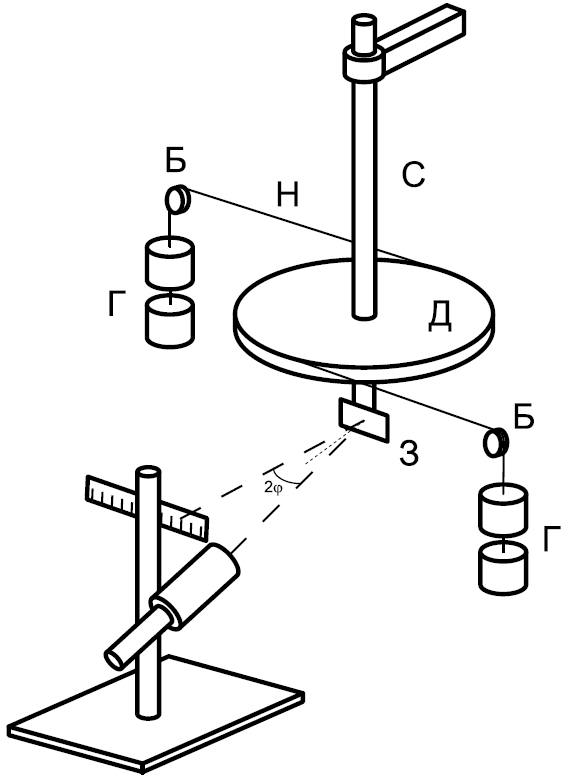
\includegraphics[scale=0.7]{ystanovka1.png}
        \begin{center}
        \caption{Схема установки}
        \end{center}
        \label{graphic1b}
    \end{center}
\end{figure}


\newpage
\subsection{Расчет всех данных}

\begin{table}[h!]
\begin{center}
\begin{tabular}{|c|c|c|}
\hline
Диаметр стержня     & $d_{\text{ст}}$, мм & 4,83 $\pm$ 0,1  \\ \hline
Диаметр диска       & $d_{\text{д}}$, мм  & 92 $\pm$ 0,1    \\ \hline
Расстояние до шкалы & $L$, см             & 140 $\pm$ 1     \\ \hline
Длина стержня       & $l$, см             & 132,8 $\pm$ 0,1 \\ \hline
Масса платформы     & $m_{0}$, гр         & 50 $\pm$ 0,01   \\ \hline
\end{tabular}
\caption{Размеры установки}
\end{center}
\end{table}

Момент силы грузов будет равен $M = (m_{1}+m_{0})gR_{\text{диск}} + (m_{2}+m_{0})gR_{\text{диск}} \approx 2(m+m_{0})gR_{\text{диск}}$.\\
Угол поворота будет равен $\varphi = arctg(\frac{\Delta l}{L}) \approx \frac{\Delta l}{L} (\Delta l \ll L)$.

\begin{table}[h!]
\begin{center}
\begin{tabular}{|c|c|c|c|}
\hline
Масса груза 1/2, $m$, гр & Момент силы, $M$, Н $\cdot$ м & Отклонение по шкале, $\Delta l$, см & Угол поворота, $\varphi$, рад \\ \hline
0                        & 0                             & 0                                   & 0                             \\ \hline
50                       & 0,09016                       & 2,6                                 & 0,018571                      \\ \hline
100                      & 0,13524                       & 3                                   & 0,021429                      \\ \hline
150                      & 0,18032                       & 6                                   & 0,042857                      \\ \hline
200                      & 0,2254                        & 8,4                                 & 0,06                          \\ \hline
250                      & 0,27048                       & 11,1                                & 0,079286                      \\ \hline
300                      & 0,31556                       & 10,85                               & 0,0775                        \\ \hline
350                      & 0,36064                       & 13,85                               & 0,098929                      \\ \hline
400                      & 0,40572                       & 15,95                               & 0,113929                      \\ \hline
\end{tabular}
\caption{Экспериментальные данные}
\end{center}
\end{table}

\newpage
\subsection{Обработка результатов}

Расчет погрешность при аппроксимации по МНК:

\[k=\frac{\langle xy\rangle-\langle x\rangle \langle y\rangle}{\langle x^2\rangle - \langle x\rangle^2}\]
\[\sigma_{k} = \frac{1}{\sqrt{N}}\sqrt{\frac{\langle y^2 \rangle - \langle y \rangle ^2}{\langle x^2 \rangle - \langle x \rangle ^2} - k^2}\]\\
Тогда $k = 0,291 \pm 0,015 (\varepsilon_{k} \approx 5,1\%)$.\\
Получаем $f = \frac{1}{k} = 3,44 \pm 0,175 (\varepsilon_{f} \approx 5,1\%)$.
\[
    G=\frac{2l}{\pi R^{4}}f
\]
Погрешность:
\[
    \varepsilon_{G} = \sqrt{(\varepsilon_{f})^2 + (\varepsilon_{l})^2 + (4\varepsilon_{R})^2} 
\]
Получаем $\varepsilon_{G} = 5,12\%$ и $G = 0,76$ ГПа

\begin{table}[h!]
\begin{center}
\begin{tabular}{|c|c|c|c|c|c|}
\hline
$\sigma_{l}$ & 0,5 см & $l$ & 141 см    & $\varepsilon_{l}$ & $0,35\%$ \\ \hline
$\sigma_{R}$ & 0,1 мм   & $R$ & 92 мм    & $\varepsilon_{R}$ & $0,1\%$  \\ \hline
$\sigma_{f}$ & 3,44 $\frac{\text{Н$\cdot$м}}{\text{рад}}$ & $f$ & 0,175 $\frac{\text{Н$\cdot$м}}{\text{рад}}$ & $\varepsilon_{f}$ & $5,1\%$ \\ \hline
\end{tabular}
\caption{Погрешности}
\end{center}
\end{table}

\begin{figure}[p]
    \centering
    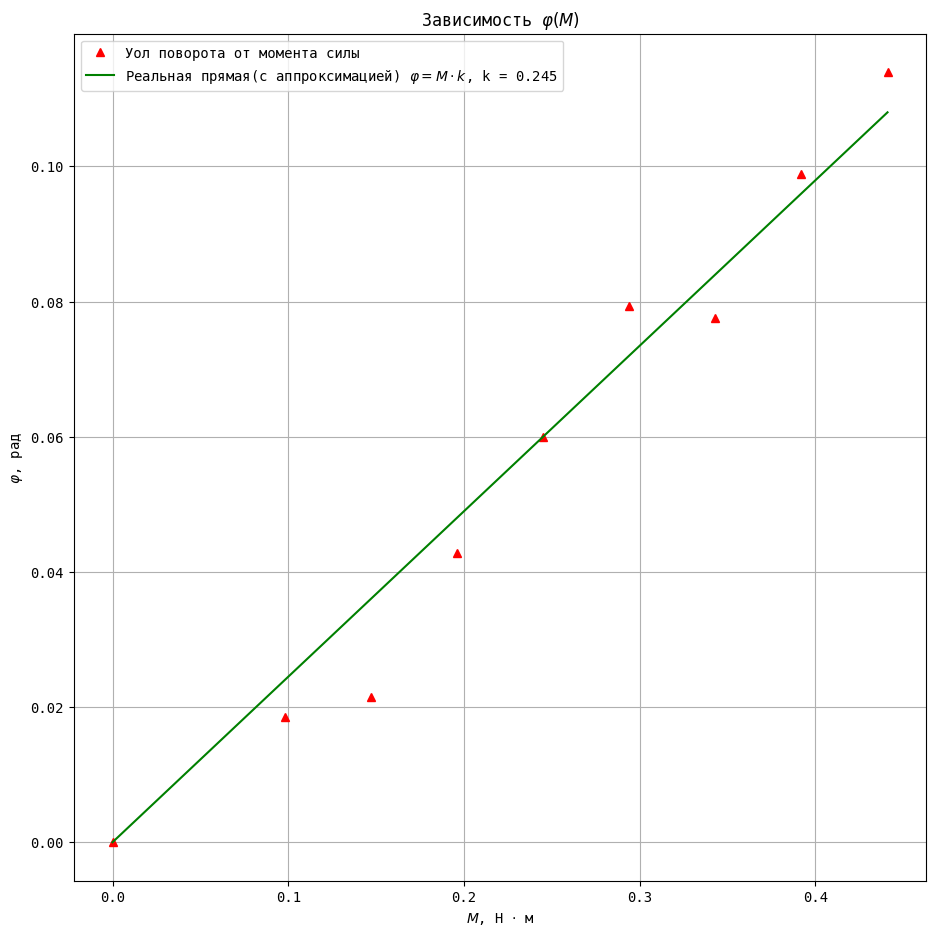
\includegraphics[scale=0.8]{graphic1.png}
    \caption{Зависимость $\varphi = k \cdot M$}
\end{figure}

\newpage
\section{Выводы}

В работе была исследована зависимость между кручением и нагрузкой.\\
Был рассчитан модуль кручения для стального стержня $G = 0,76 \pm 0,039 (\varepsilon_{G} = 5,12\%)$ ГПа. Полученное значение лежит в пределах одного $\sigma_{G}$ при сравнении с табличным значением.

\newpage
\section{Определение модуля сдвига при помощи крутильных колебаний}

\subsection{Теоретическая часть}

В системе можно возбудить крутильные колебания. Вращение стержня с закрепленными
на нем грузиками вокрунг вертикальной оси проиходит под действием упругого момента $M$.
С учетом выражения для момента $M$ получим, что это вращение описывается уравнением колебаний:
\begin{equation}
    I\frac{d^2 \varphi }{d t^2} + f \varphi =0
\end{equation}
Следовательно период кoлебаний системы связан с расстоянием $r$ от оси вращения до грузов и
моментом инерции стержня $I_0$ следующим образом:
\begin{equation}
    \omega^2 = \frac{f}{I}
\end{equation}

\begin{equation}
    T = 2\pi\sqrt{\frac{I}{f}}
\end{equation}
Эти зависимости были получены для незатухающих колебаний. Поэтому для их применения необходимо убедиться, что в рассматриваемой системе диссипативными силами можно пренебречь. Для этого стоит убедиться, что период колебаний не зависит от начальной амплитуды и что амплитуда уменшьется не более чем в 2 раза после около 10 колебаний.\\
Применяя Теорему Гюйгенса-Штейнера
\begin{equation}
    T^2 = (2\pi)^2\frac{I}{f} = (2\pi)^2\frac{I_{0}}{f} + (2\pi)^2\frac{(m_{1}+m_{2})r^2}{f}
\end{equation}
,где $I_{0} = \frac{1}{4}mr^2 + \frac{1}{12}ml^2 + \frac{1}{4}ml^2 = \frac{1}{4}mr^2 + \frac{1}{3}ml^2$

\subsection{Экспериментальная установка}

Экспериментальная установка, используемая в этой части работы,
изображена на рис. 1 и состоит из длинной вертикально висящей право-
локи П, к нижнему концу которой прикреплен горизонтальный метал-
лический стержень С с двумя симметрично расположенными грузами
Г. Их положение на стержне можно фиксировать. Верхний конец право-
локи зажать в цангу и при помощи специального приспособления может
вместе с цангой поворачиваться вокруг вертикальной оси. Таким спо-
собом в системе можно возбуждать крутильные колебания. Вращение
стержня С с закрепленными на нем грузами Г вокруг вертикальной
оси происходит под действием упругого момента, возникающего в проволоке.

\begin{figure}[!h]
    \begin{center}
        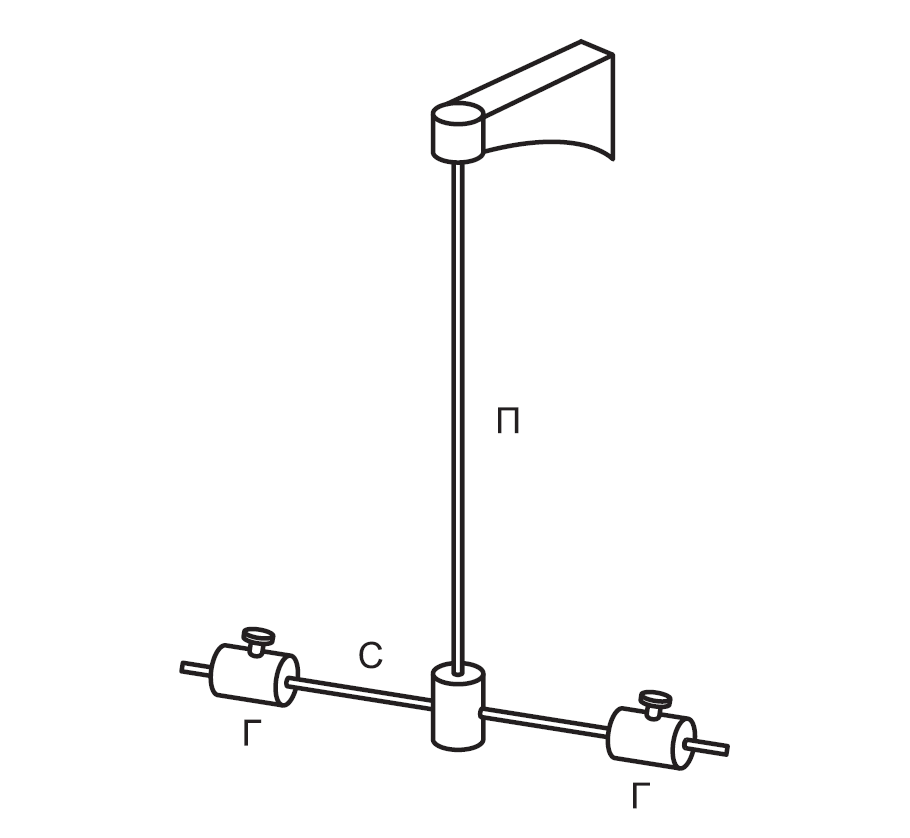
\includegraphics[scale=0.7]{ystanovka2.png}
        \begin{center}
        \caption{Схема установки}
        \end{center}
        \label{graphic1b}
    \end{center}
\end{figure}

\newpage
\subsection{Расчет всех данных}

\begin{table}[h!]
\begin{center}
\begin{tabular}{|c|c|}
\hline
Масса груза 1, гр     & 202,5 $\pm$ 0,1 \\ \hline
Масса груза 2, гр     & 204,1 $\pm$ 0,1 \\ \hline
Диаметр проволоки, мм & 1,39 $\pm$ 0,01 \\ \hline
Длина проволоки, мм   & 1730 $\pm$ 2    \\ \hline
Длина цилиндра, мм    & 48 $\pm$ 0,1    \\ \hline
\end{tabular}
\caption{Размеры установки}
\end{center}
\end{table}

\begin{table}[h!]
\begin{center}
\begin{tabular}{|c|c|}
\hline
$l$, см & Период, $T$, с \\ \hline
5,8  & 1,623 \\ \hline
6,8  & 1,666 \\ \hline
7,8  & 1,732 \\ \hline
8,8  & 1,81  \\ \hline
9,8  & 1,867 \\ \hline
10,8 & 1,974 \\ \hline
11,8 & 2,065 \\ \hline
12,8 & 2,177 \\ \hline
13,8 & 2,26  \\ \hline
14,8 & 2,357 \\ \hline
\end{tabular}
\caption{Экспериментальные данные}
\end{center}
\end{table}

\newpage
\subsection{Обработка результатов}

\begin{equation}
    T^2 = (2\pi)^2\frac{I}{f} = (2\pi)^2\frac{I_{0}}{f} + (2\pi)^2\frac{(m_{1}+m_{2})r^2}{f}
\end{equation}
,где $I_{0} = \frac{1}{4}mr^2 + \frac{1}{12}ml^2 + \frac{1}{4}ml^2 = \frac{1}{4}mr^2 + \frac{1}{3}ml^2$\\

Расчет погрешность при аппроксимации по МНК:

\[k=\frac{\langle xy\rangle-\langle x\rangle \langle y\rangle}{\langle x^2\rangle - \langle x\rangle^2}\]
\[\sigma_{k} = \frac{1}{\sqrt{N}}\sqrt{\frac{\langle y^2 \rangle - \langle y \rangle ^2}{\langle x^2 \rangle - \langle x \rangle ^2} - k^2}\]\\
Тогда $k = 0,065 \pm  0,00089 (\varepsilon_{k} \approx 1,35\%)$ $\frac{c^2}{\text{см}^2}$.\\
\begin{align}
    k &= (2\pi)^2\frac{(m_{1}+m_{2})}{f}\\
    f &= (2\pi)^2\frac{(m_{1}+m_{2})}{k}
\end{align}
Погрешность:
\[
    \varepsilon_{f} = \sqrt{(\varepsilon_{m_{1}})^2 + (\varepsilon_{m_{2}})^2 + (\varepsilon_{k})^2} 
\]
Получаем $\varepsilon_{f} = 1,35\%$ и $f = 0,0247$ Н $\cdot$ м.\\
\[
    G=\frac{2l}{\pi R^{4}}f
\]
Погрешность:
\[
    \varepsilon_{G} = \sqrt{(\varepsilon_{f})^2 + (\varepsilon_{l})^2 + (4\varepsilon_{R})^2} 
\]
Получаем $\varepsilon_{G} = 3,16\%$ и $G = 11,5 \cdot 10^{10} \frac{\text{Н}}{\text{м}^2}$ 

\begin{table}[h!]
\begin{center}
\begin{tabular}{|c|c|c|c|c|c|}
\hline
$\sigma_{m_{1}}$ & 0,1 гр & $m_{1}$ & 202,5 гр    & $\varepsilon_{m_{1}}$ & $0,05\%$ \\ \hline
$\sigma_{m_{2}}$ & 0,1 гр   & $m_{2}$ & 204,1 гр    & $\varepsilon_{m_{2}}$ & $0,05\%$  \\ \hline
$\sigma_{k}$ & 0,00089 $\frac{c^2}{\text{см}^2}$ & $k$ & 0,065 $\frac{c^2}{\text{см}^2}$ & $\varepsilon_{k}$ & $1,3\%$ \\ \hline
$\sigma_{l}$ & 2 мм   & $l$ & 1730 мм    & $\varepsilon_{l}$ & $0,11\%$  \\ \hline
$\sigma_{R}$ & 0,005 мм   & $R$ & 0,695 мм    & $\varepsilon_{R}$ & $0,72\%$  \\ \hline
\end{tabular}
\caption{Погрешности}
\end{center}
\end{table}

\begin{figure}[p]
    \centering
    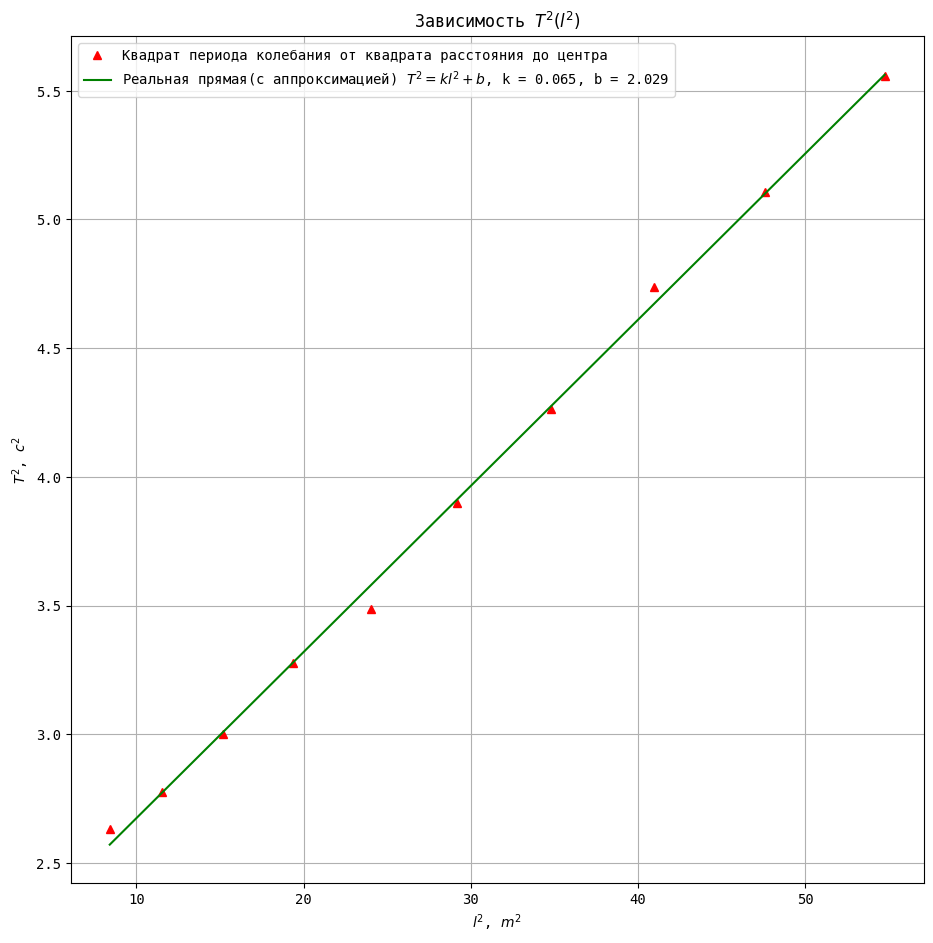
\includegraphics[scale=0.8]{graphic2.png}
    \caption{Зависимость $T^2 = kl^2 + b$}
\end{figure}

\newpage
\section{Выводы}
В работе была исследована зависимость между кручением и нагрузкой.\\
Был рассчитан модуль кручения для стального стержня $G = 11,5 \pm 0,36 \cdot 10^{10} (\varepsilon_{G} = 3,16\%)$ ГПа. Полученное значение лежит в пределах одного $\sigma_{G}$ при сравнении с табличным значением.

\end{document}
